\documentclass{article}
\usepackage{graphicx} % Required for inserting images

\title{CallFeedbackApp Design Doc}
\author{Gaurav Kumar \\ Shiv Narang}
\date{January 2026}

\begin{document}

\maketitle


\section{Overall Architecture}

The system follows a client--server architecture:
\begin{itemize}
    \item The \textbf{Android client} monitors call state changes and presents a feedback interface after call termination.
    \item The \textbf{Backend service} receives feedback data, validates it, and stores it for analysis and visualization.
\end{itemize}

The design emphasizes minimal user interaction, low overhead during calls, and reliable metadata collection.

\section{User Interface Design}
The mobile application provides an overlay-based feedback interface that appears after a call ends. The UI is designed to be minimal, non-intrusive, and easily dismissible.

\begin{figure}[h]
    \centering
    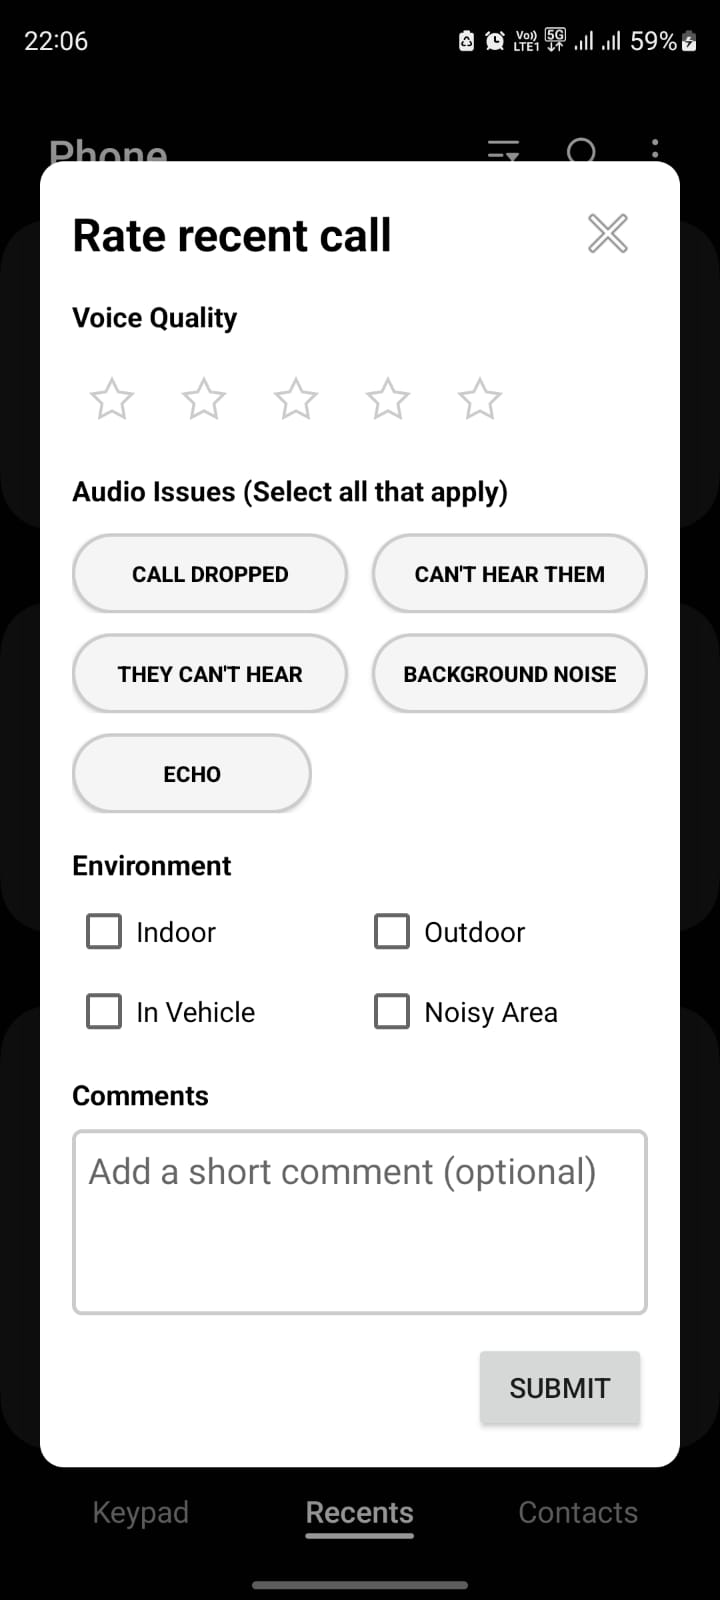
\includegraphics[width=0.35\textwidth]{overlay_ui.jpg}
    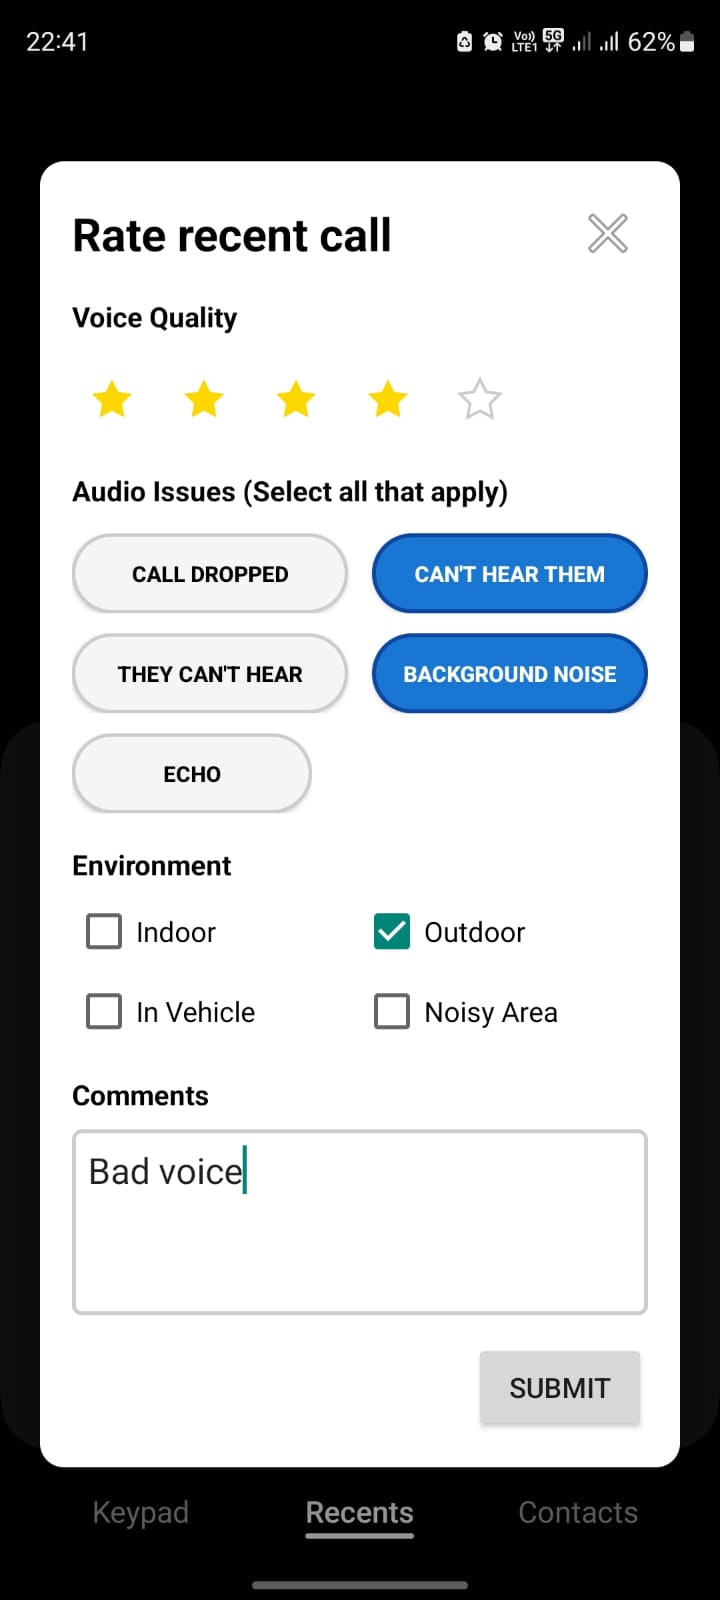
\includegraphics[width=0.35\textwidth]{feedback_activity.jpeg}
    \caption{User interface flow: overlay feedback and detailed feedback screen}
    \label{fig:ui_flow}
\end{figure}

\subsection{User Interface Flow}
The Android application continuously listens to telephony call state changes using the \texttt{TelephonyManager} API. When a transition from \texttt{CALL\_STATE\_OFFHOOK} to \texttt{CALL\_STATE\_IDLE} is detected, the system infers that a call has ended and triggers the feedback flow.

This event-driven approach ensures that the feedback UI is displayed only after the call is completed, avoiding user interruption during the call.

\subsection{Feedback Screen Layout}

The feedback interface is designed to be simple, fast, and easily accessible. The layout consists of:

\begin{itemize}
    \item A prominent heading indicating that feedback is requested.
    \item Star-based rating components for quantitative feedback such as voice quality.
    \item Optional categorical selections for audio issues and call environment.
    \item A submit button to send feedback to the backend.
\end{itemize}

Star ratings are intentionally sized larger than default UI components to improve touch accuracy and encourage user participation.

\subsection{User Interaction Flow}

The interaction flow is as follows:
\begin{enumerate}
    \item Call ends and call state listener is triggered.
    \item Feedback activity or bottom sheet is launched.
    \item User provides ratings and optional inputs.
    \item Feedback data is submitted asynchronously.
    \item UI closes automatically upon successful submission.
\end{enumerate}

All input fields are optional to minimize friction and prevent feedback abandonment.

\subsection{Metadata Collection}

Alongside user input, the client automatically collects device and network metadata at the time of feedback submission, including:
\begin{itemize}
    \item Network type (WiFi, 2G, 3G, 4G, 5G).
    \item Signal strength in dBm.
    \item Approximate geographic location (if permission is granted).
    \item Timestamp of feedback submission.
\end{itemize}

This data is collected transparently without additional user interaction.

\section{Backend Design}

\subsection{Backend Architecture}

The backend is implemented as a RESTful web service using \texttt{FastAPI}. It follows a modular architecture consisting of:

\begin{itemize}
    \item API layer for request handling.
    \item Validation layer using \texttt{Pydantic}.
    \item Persistence layer for database operations.
\end{itemize}

This separation improves maintainability, scalability, and testability.

\subsection{API Design}

The backend exposes endpoints for:
\begin{itemize}
    \item Submitting new feedback records.
    \item Retrieving stored feedback with pagination support.
\end{itemize}

All incoming requests are validated against predefined schemas to ensure data consistency and prevent malformed inputs.

\subsection{Data Model}

Feedback data is represented using structured schemas that combine:
\begin{itemize}
    \item Subjective user feedback (ratings, issues, environment).
    \item Objective device metadata (network type, signal strength, location).
\end{itemize}

Enumerations are used for categorical fields to enforce consistency across all submissions.

\subsection{Data Validation and Constraints}

The backend enforces the following constraints:
\begin{itemize}
    \item Rating values are restricted to a fixed range (1--5).
    \item Enumerated fields accept only predefined values.
    \item Optional fields allow partial submissions without rejection.
\end{itemize}

This ensures high-quality data suitable for downstream analysis.

\subsection{Storage and Retrieval}

Each feedback record is stored with a unique identifier and server-generated timestamp. Feedback retrieval supports pagination to efficiently handle large datasets, enabling scalable analytics and visualization.

\subsection{Security and Privacy Considerations}

The system is designed with privacy in mind:
\begin{itemize}
    \item No call audio or phone numbers are recorded.
    \item Location data is collected only when permission is granted.
    \item All communication occurs over secure HTTP (HTTPS).
\end{itemize}

User participation is voluntary, and feedback submission does not block normal phone usage.

\section{Design Rationale}

The combined UI and backend design prioritizes:
\begin{itemize}
    \item Low user effort and minimal disruption.
    \item Accurate correlation between perceived quality and network conditions.
    \item Extensibility for future metrics and analytics.
\end{itemize}

This design makes the system suitable for large-scale network performance research and real-world deployment.

\end{document}
